\section{Theory of small on large}
Initially proposed by Humphrey in \cite{Baek}, the theory of small on large is an idea to impose a computational process with small characteristic time to a process with large characteristic time. In this method, FSI and the growth are computed alternately with different time steps. To solve the FSI with small time step, the growth is frozen based on the assumption that the growth process is too slow to have a significant effect during a few seconds. Once the FSI computation finishes, an average load of the fluid to the solid tissue could be obtained and used as the external load in the growth simulation, which uses a much larger time step. Notice in the computation of the growth, the change of the external load is neglected since the average load from the previous FSI cycle is used.

Denote the current and next time steps of in the growth model as $t_\mathrm{n}$ and $t_\mathrm{n+1}$. Take a long, straight vessel as an example, the process of the theory of small on large can be illustrated as Figure \ref{fig:smallOnLarge}:
\begin{figure}[H]
   \centering
   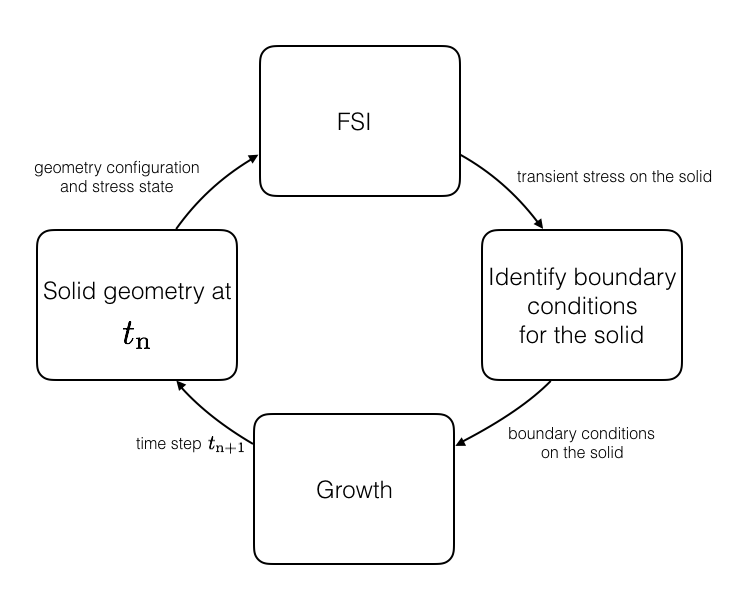
\includegraphics[width=.6\textwidth]{./figures/smallOnLarge.png} % requires the graphicx package
   \caption{Iteration and the information passing in the theory of small on large}
   \label{fig:smallOnLarge}
\end{figure}

The effect of the fluid on the solid is classified as the hydrostatic pressure $p(\bX)$ and wall shear stress $\tau(\bx)$ which are functions of the undeformed coordinates $\bX$. Let $T$ be the computational period of the FSI process, the average pressure $\bar{p}(\bX)$ and wall shear stress $\bar{\boldsymbol{\tau}}(\bX)$ can be obtained as:
\begin{subequations}
\begin{align}
\bar{p}(\bX) &= \frac{1}{T}\int_0^T p(\bX) dt\\
\bar{\boldsymbol{\tau}}(\bX) &= \frac{1}{T}\int_0^T \boldsymbol{\tau}(\bX) dt
\end{align}
\end{subequations}

In \cite{Figueroa}, the theory of small on large was applied with the theory of mixtures which models the arterial wall as a constrained mixture of amorphous elastin matrix, collagen fibers and smooth muscle. In this constrained mixture theory, the growth seeks to maintain a homeostatic biomechanical state via reorganizing and replacing existing constituents with new constituents that have different orientations or mass fractions but identical mechanical properties. In general, the mixture theory may overlook phenomena that can play important biological roles and the role of osmotic pressure \cite{Ambrosi}. Furthermore, although the mixture theory is a self-consistent system, it depends on multiple empirical parameters and is difficult to be combined into finite element framework. Theses factors significantly hinder the application of the mixture theory. The multiplicative growth model used in our research, however, is much more flexible. Not only it allows for different ways to control the growth, but also it can be easily implemented in the existing finite element framework. Combining the theory of small on large with the multiplicative growth model allows us to account for the fluid-structure interaction during the biological growth without the disadvantages of the original content of mixture theory.